%% 
%% Copyright 2007-2020 Elsevier Ltd
%% 
%% This file is part of the 'Elsarticle Bundle'.
%% ---------------------------------------------
%% 
%% It may be distributed under the conditions of the LaTeX Project Public
%% License, either version 1.2 of this license or (at your option) any
%% later version.  The latest version of this license is in
%%    http://www.latex-project.org/lppl.txt
%% and version 1.2 or later is part of all distributions of LaTeX
%% version 1999/12/01 or later.
%% 
%% The list of all files belonging to the 'Elsarticle Bundle' is
%% given in the file `manifest.txt'.
%% 
%% Template article for Elsevier's document class `elsarticle'
%% with harvard style bibliographic references

\documentclass[preprint,12pt,authoryear]{elsarticle}

%% Use the option review to obtain double line spacing
%% \documentclass[authoryear,preprint,review,12pt]{elsarticle}

%% Use the options 1p,twocolumn; 3p; 3p,twocolumn; 5p; or 5p,twocolumn
%% for a journal layout:
%% \documentclass[final,1p,times,authoryear]{elsarticle}
%% \documentclass[final,1p,times,twocolumn,authoryear]{elsarticle}
%% \documentclass[final,3p,times,authoryear]{elsarticle}
%% \documentclass[final,3p,times,twocolumn,authoryear]{elsarticle}
%% \documentclass[final,5p,times,authoryear]{elsarticle}
%% \documentclass[final,5p,times,twocolumn,authoryear]{elsarticle}

%% For including figures, graphicx.sty has been loaded in
%% elsarticle.cls. If you prefer to use the old commands
%% please give \usepackage{epsfig}

%% The amssymb package provides various useful mathematical symbols
\usepackage{amssymb}
%% The amsthm package provides extended theorem environments
%% \usepackage{amsthm}

%% The lineno packages adds line numbers. Start line numbering with
%% \begin{linenumbers}, end it with \end{linenumbers}. Or switch it on
%% for the whole article with \linenumbers.
%% \usepackage{lineno}

\journal{Geoenergy Science and Engineering}

\begin{document}

\begin{frontmatter}

%% Title, authors and addresses

%% use the tnoteref command within \title for footnotes;
%% use the tnotetext command for theassociated footnote;
%% use the fnref command within \author or \affiliation for footnotes;
%% use the fntext command for theassociated footnote;
%% use the corref command within \author for corresponding author footnotes;
%% use the cortext command for theassociated footnote;
%% use the ead command for the email address,
%% and the form \ead[url] for the home page:
%% \title{Title\tnoteref{label1}}
%% \tnotetext[label1]{}
%% \author{Name\corref{cor1}\fnref{label2}}
%% \ead{email address}
%% \ead[url]{home page}
%% \fntext[label2]{}
%% \cortext[cor1]{}
%% \affiliation{organization={},
%%            addressline={}, 
%%            city={},
%%            postcode={}, 
%%            state={},
%%            country={}}
%% \fntext[label3]{}

\title{Oil and gas production forecasting using XGBoost regressor}

%% use optional labels to link authors explicitly to addresses:
%% \author[label1,label2]{}
%% \affiliation[label1]{organization={},
%%             addressline={},
%%             city={},
%%             postcode={},
%%             state={},
%%             country={}}
%%
%% \affiliation[label2]{organization={},
%%             addressline={},
%%             city={},
%%             postcode={},
%%             state={},
%%             country={}}
\author[inst1]{Vinicius Mattoso R. da Silva}

\affiliation[inst1]{organization={Laboratory of Microhydrodynamics and Flow in Porous Media, Pontifical Catholic University of Rio de Janeiro (PUC-Rio)},%Department and Organization
            % addressline={Address Two}, 
            % city={Rio de Janeiro},
            % postcode={22222}, 
            state={Rio de Janeiro},
            country={Brazil}}

\author[inst1]{Frederico Gomes}
\author[inst1]{Sergio Ribeiro}
\author[inst1]{Marcio Carvalho}

\begin{abstract}

% The oil and gas industry has a vital role in the global economy. Due to the financial impact, an efficient operation is a target that many companies look for. With the capability to predict the production of oil and gas, companies are able to optimize their operations and costs, improving their operational efficiency more and more. In order to overcome this issue, many companies use reservoir simulation software to predict production. Nonetheless, this approach to solving the problem requires a huge computational cost and a reliable geological model. Both of the requirements are expensive, and a reliable geological model of the reservoir is another issue that the industry has. With the advantage of artificial intelligence resources, companies can use their owners' amount of data in order to make data-driven models to overcome many industries' issues, including the production forecast. In this study, a machine learning model was used to predict the oil and gas production from a wellbore, making use of the time series from the sensors along the wellbore regions. The results showed the relevance of the feature engineering process and the capability of the model to predict oil and gas based on the available data.

% V2

The world economy greatly depends on the oil and gas industry. An efficient operation is a goal that many firms pursue due to its financial impact. Companies are able to optimize their production and costs, increasing their operational efficiency as a result of their ability to predict the production of oil and gas. Many businesses employ reservoir simulation software to forecast production to get around this problem. However, this method of issue-solving necessitates a solid geological model and a high computing cost. Both of the requirements are expensive, and the sector also faces a problem with a trustworthy geological model of the reservoir. With the use of artificial intelligence resources, businesses can take advantage of the vast amounts of data that belong to their owners to create data-driven models that address problems common to many industries, such as production forecasting. The data series from the sensors along the wellbore areas were utilized in this study to train a machine-learning model to forecast the oil and gas output from a wellbore. The outcomes demonstrated the applicability of the feature engineering procedure and the model's capacity to forecast oil and gas based on the available data.


% The forecast of oil and gas production is essential for the industry's efficient operation.


% Forecasting oil and gas production is essential for the industry to operate efficiently. Companies can optimize their operations, streamline costs, and remain competitive by accurately predicting production levels. In the past, predicting production levels was a challenging task that relied on historical data and intuition. Still, with the advancement of machine learning models such as XGBoost, companies can now make data-driven decisions and leverage the power of predictive analytics to gain a competitive edge. The relevance of forecasting in the oil and gas industry cannot be overstated, and accurate predictions are crucial for maintaining profitability and ensuring sustainable growth.


\end{abstract}

%%Graphical abstract
\begin{graphicalabstract}
%\includegraphics{grabs}
\end{graphicalabstract}

%%Research highlights
\begin{highlights}
\item Research highlight 1
\item Research highlight 2
\end{highlights}

\begin{keyword}
%% keywords here, in the form: keyword \sep keyword
Production forecasting, \ Machine learning, \ Tree boosting, regressor, \ Data-driven model
%% PACS codes here, in the form: \PACS code \sep code

%% MSC codes here, in the form: \MSC code \sep code
%% or \MSC[2008] code \sep code (2000 is the default)

\end{keyword}

\end{frontmatter}

%% \linenumbers

%% main text
\section{Introduction}
\label{sec:Introduction}
% The oil and gas industry has a huge relevance in people's life. This business surrounds humans in the means of locomotion, as a thermal source, providing raw material for several other industries. Due to its importance, its production has great relevance in the world economy.

The oil and gas industry provides fuel for locomotion and thermal sources, it also provides raw materials for several other industries.
Due to its relevance in human life, its production has great relevance in the world economy.



In addition to applications for phase identification, AI techniques can also be found in forecasting works such as Nait Amar and Zerabi\cite{nait2020combined}, in which the downhole pressure prediction was made, and there are also works forecast of hydrocarbon production (\cite{cao2016data}, \cite{zanjani2020data}).

Aiming precisely to facilitate future production planning, this work used a machine learning model to learn the relationship between the volumes of each phase produced and other information from sensors coupled to the well. With a properly trained model, we are able to make predictions of the production volume of each phase produced based on information from the sensors. The model used was $extreme gradient boost$ (XGBoost)\cite{chen2016xgboost} which is a machine learning model with supervised learning, which has been applied by several works to make predictions in different areas such as sales forecasts (\cite{shilong2021machine} ) and oil price forecasts ( \cite{gumus2017crude}).

This work structure starts with a brief explanation of the dataset used with the respective considerations about the variables used to build the model, then the methodology used to make the model, followed by the results, and finally the conclusions of the work.

\section{Dataset: evaluations and preparations}
\label{sec:InformationsAndAvaliations}

For the development of this work, real field data were used. The data was provided by \cite{equinor2018volve} and is from the Volve field in the Norwegian continental shelf (NCS). This field was discovered in 1993 and it is located in the central part of the North Sea. The production of the field started in 2008. The image above is a crop from the NCS map with contains the Volve field domain, this image was taken from the Norwegian Petroleum \cite{directorate2017factpages}.

\begin{figure}[h!]
    \centering
    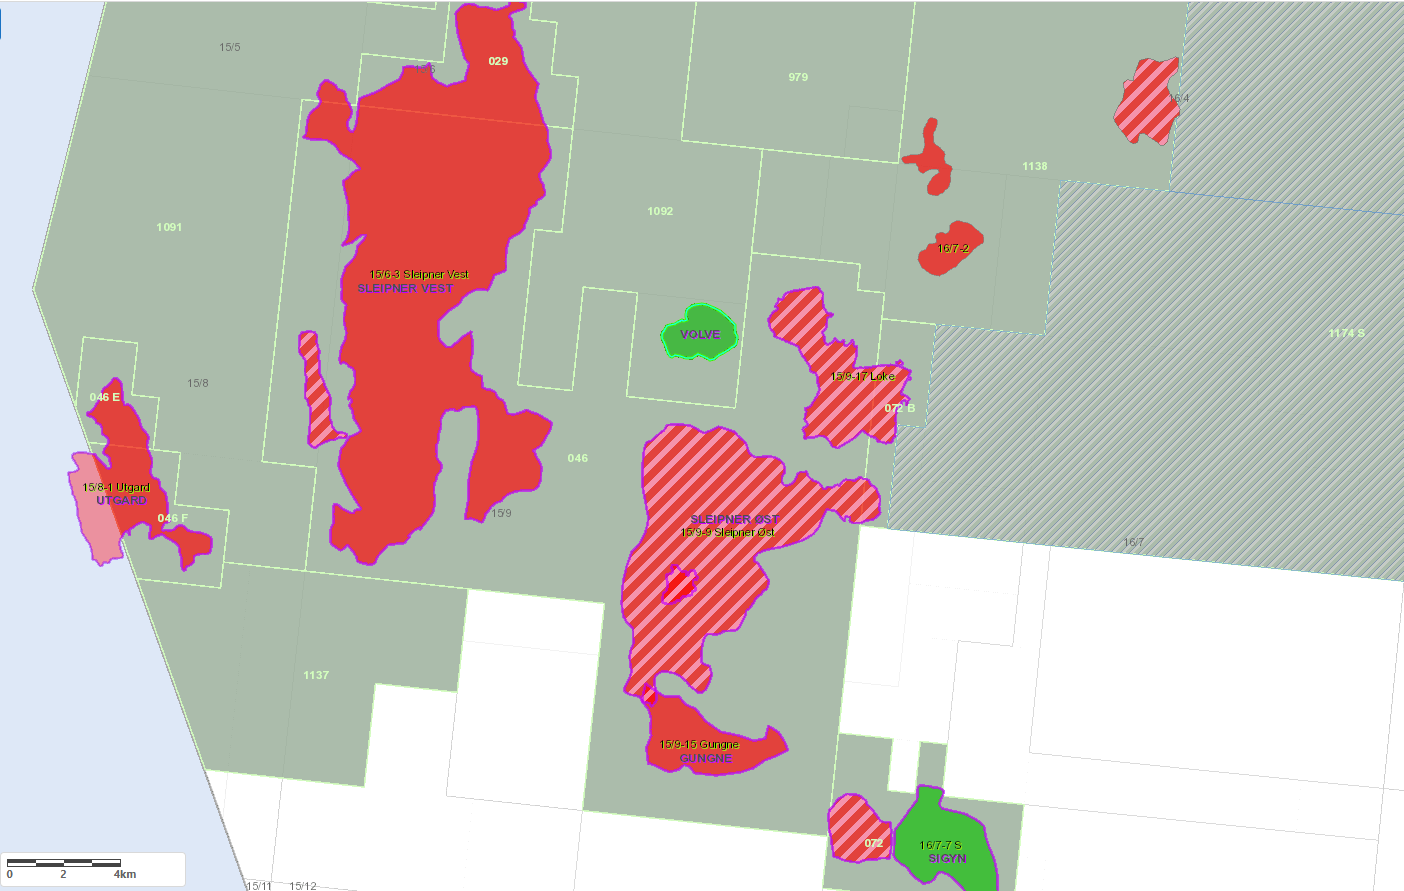
\includegraphics[width=1.0\textwidth]{images/volve_field_my.png}
    \caption{crop from the NCS map that contains the Volve field domain.}
    \label{fig:volve_field}
\end{figure}

In the dataset provided by \cite{equinor2018volve}, there are different types of data such as production data, geological information, reservoir modeling, seismic, and others. This work is focused on the production data, but there are other works such as \cite{sen2019estimation}, and \cite{ravasi2015vector} that contain information about the other available data.

The production dataset contains information that is crucial for planning future activities and understanding the behavior of the field. The file has information about the injections, productions, and observations wells that compose the field. In this work, was used the productor well with the code NO15-9-F-12-H. Figure \ref{fig:all_features} display the different time series that are available in the dataset.

Despite the average from the downhole pressure (\emph{$avg\_downhole\_pressure$}) and the average from the downhole temperature (\emph{$avg\_downhole\_temperature$}) being available data, it is notable in fig \ref{fig:all_features} that from point 1000 onwards both series remain at zero without showing any variation, this behavior is not consistent with the physics present in the production process or during well closure. Therefore, both series were removed from the machine learning model training process.




% \begin{figure}[h!]
%     \centering
%     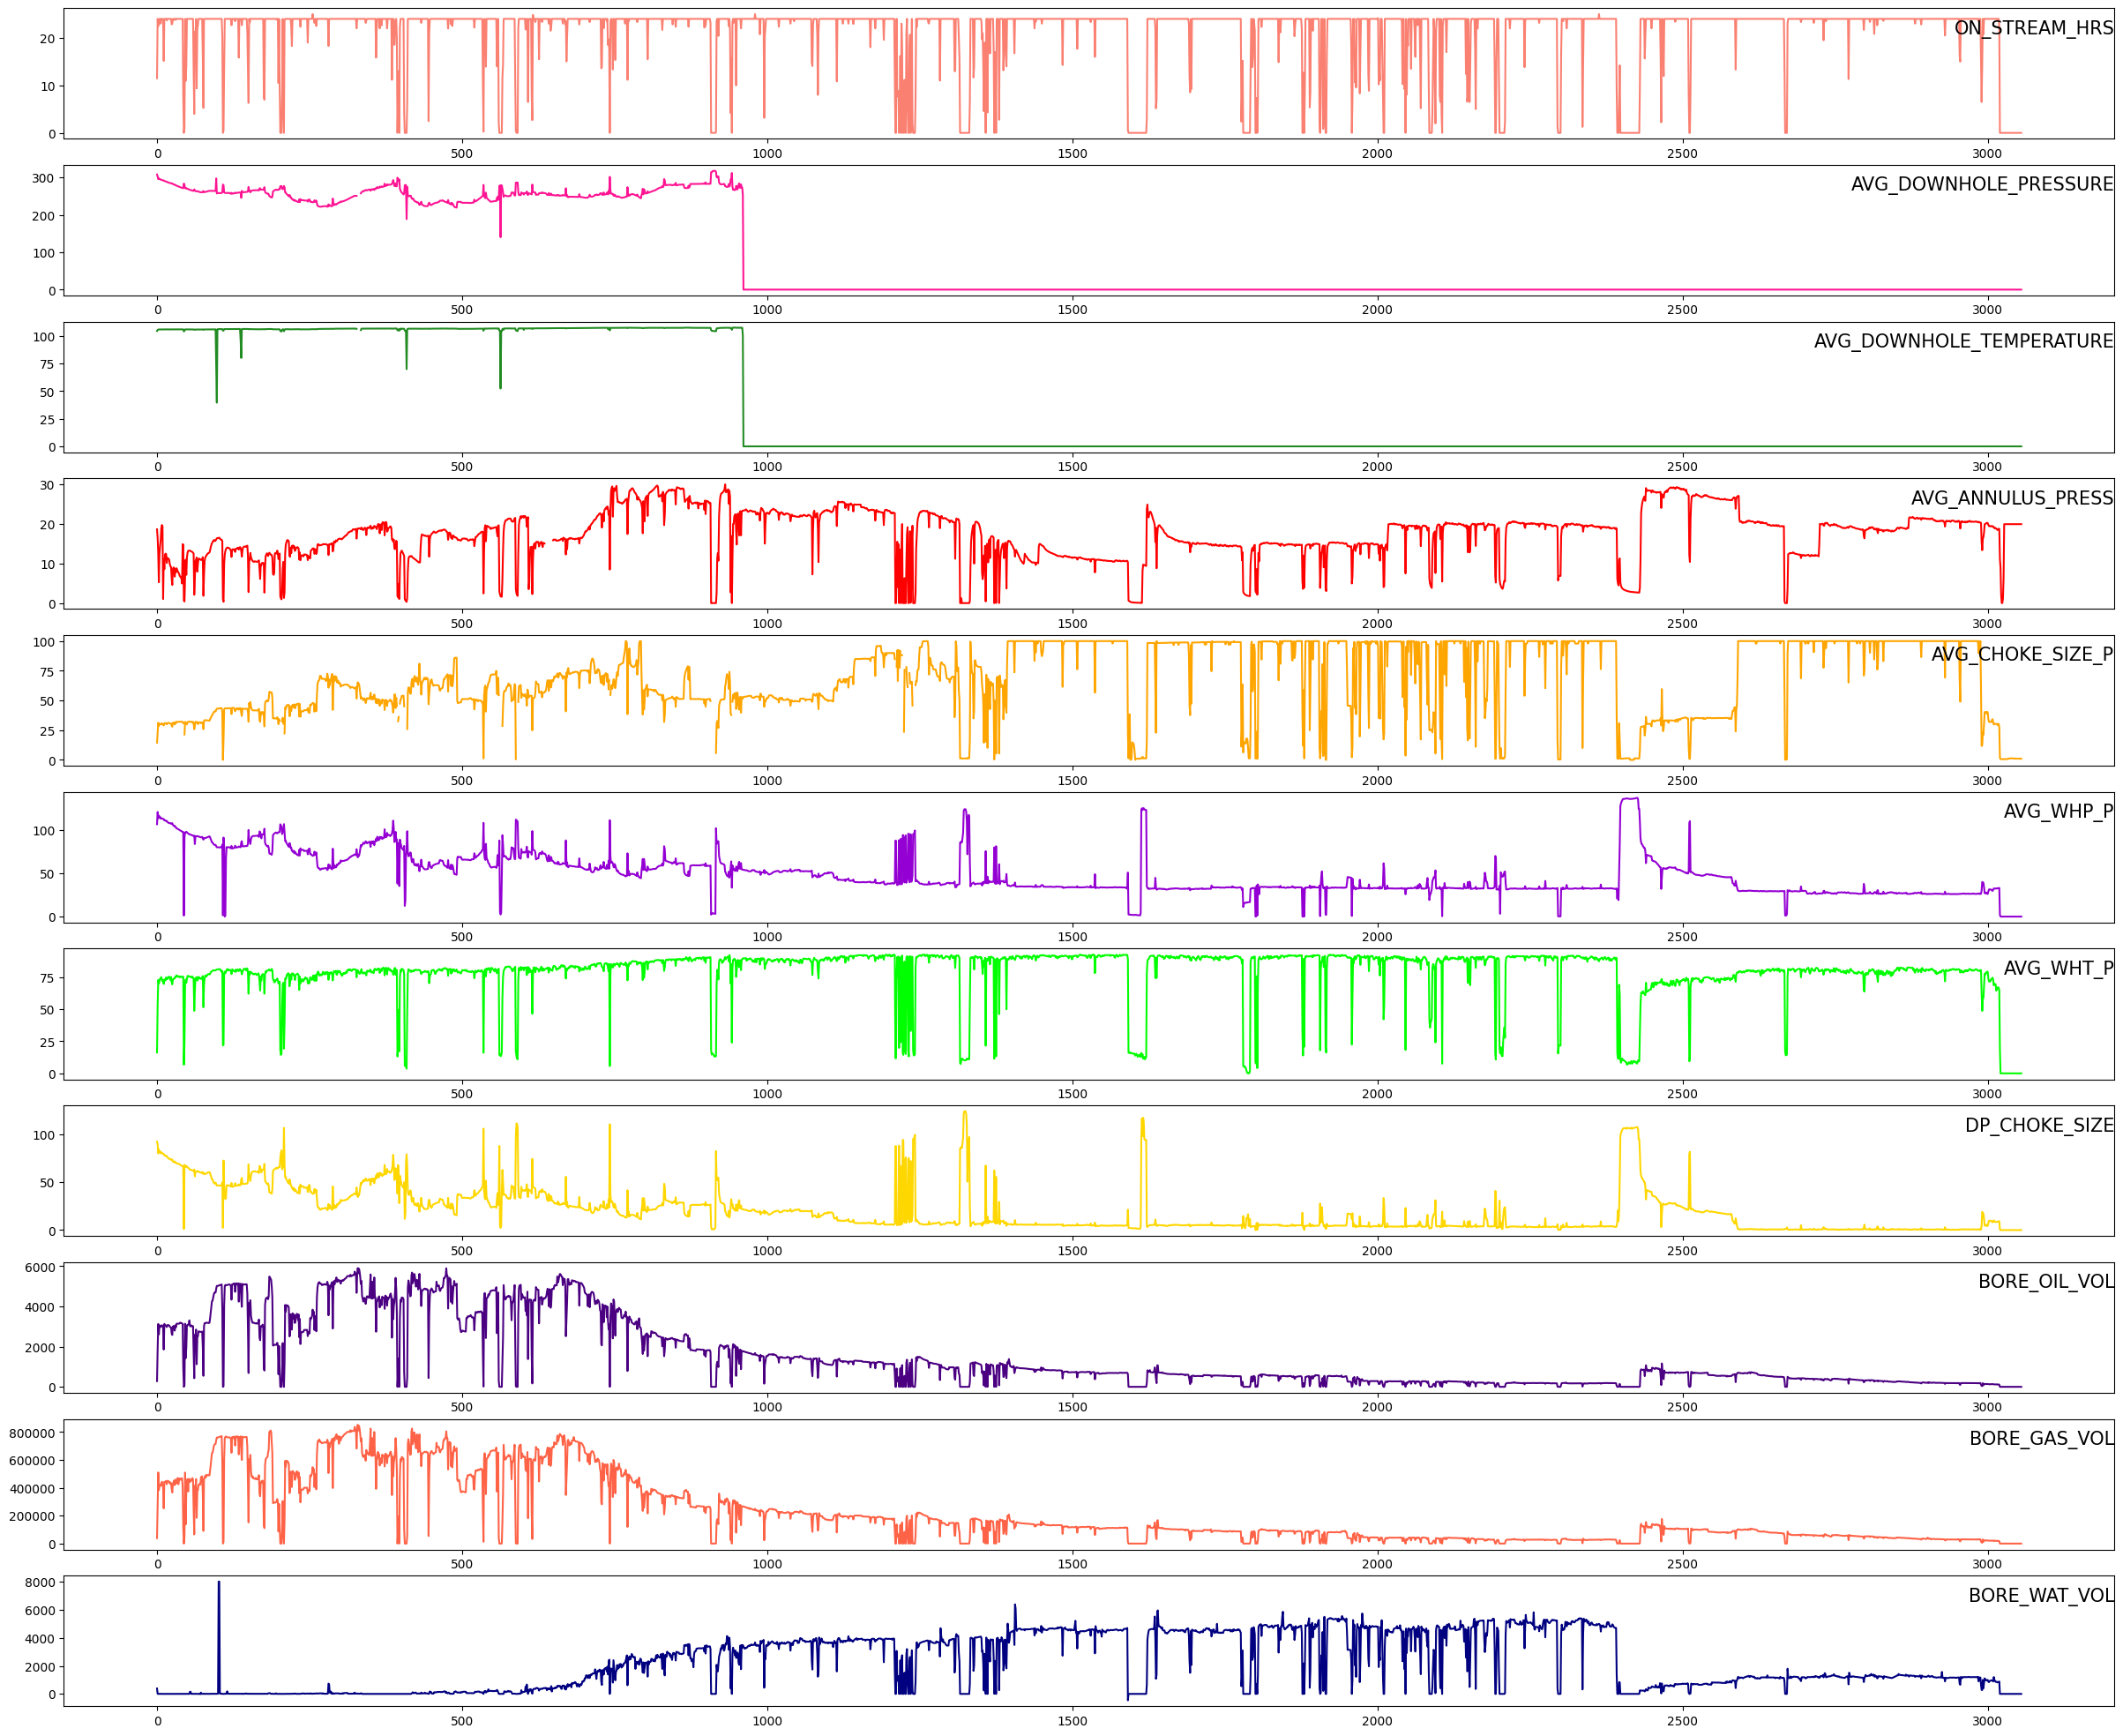
\includegraphics[width=1.0\textwidth]{images/all_features.png}
%     \caption{Time series available to be used in the forecasting process.}
%     \label{fig:all_features}
% \end{figure}

\begin{figure}[h!]
    \centering
    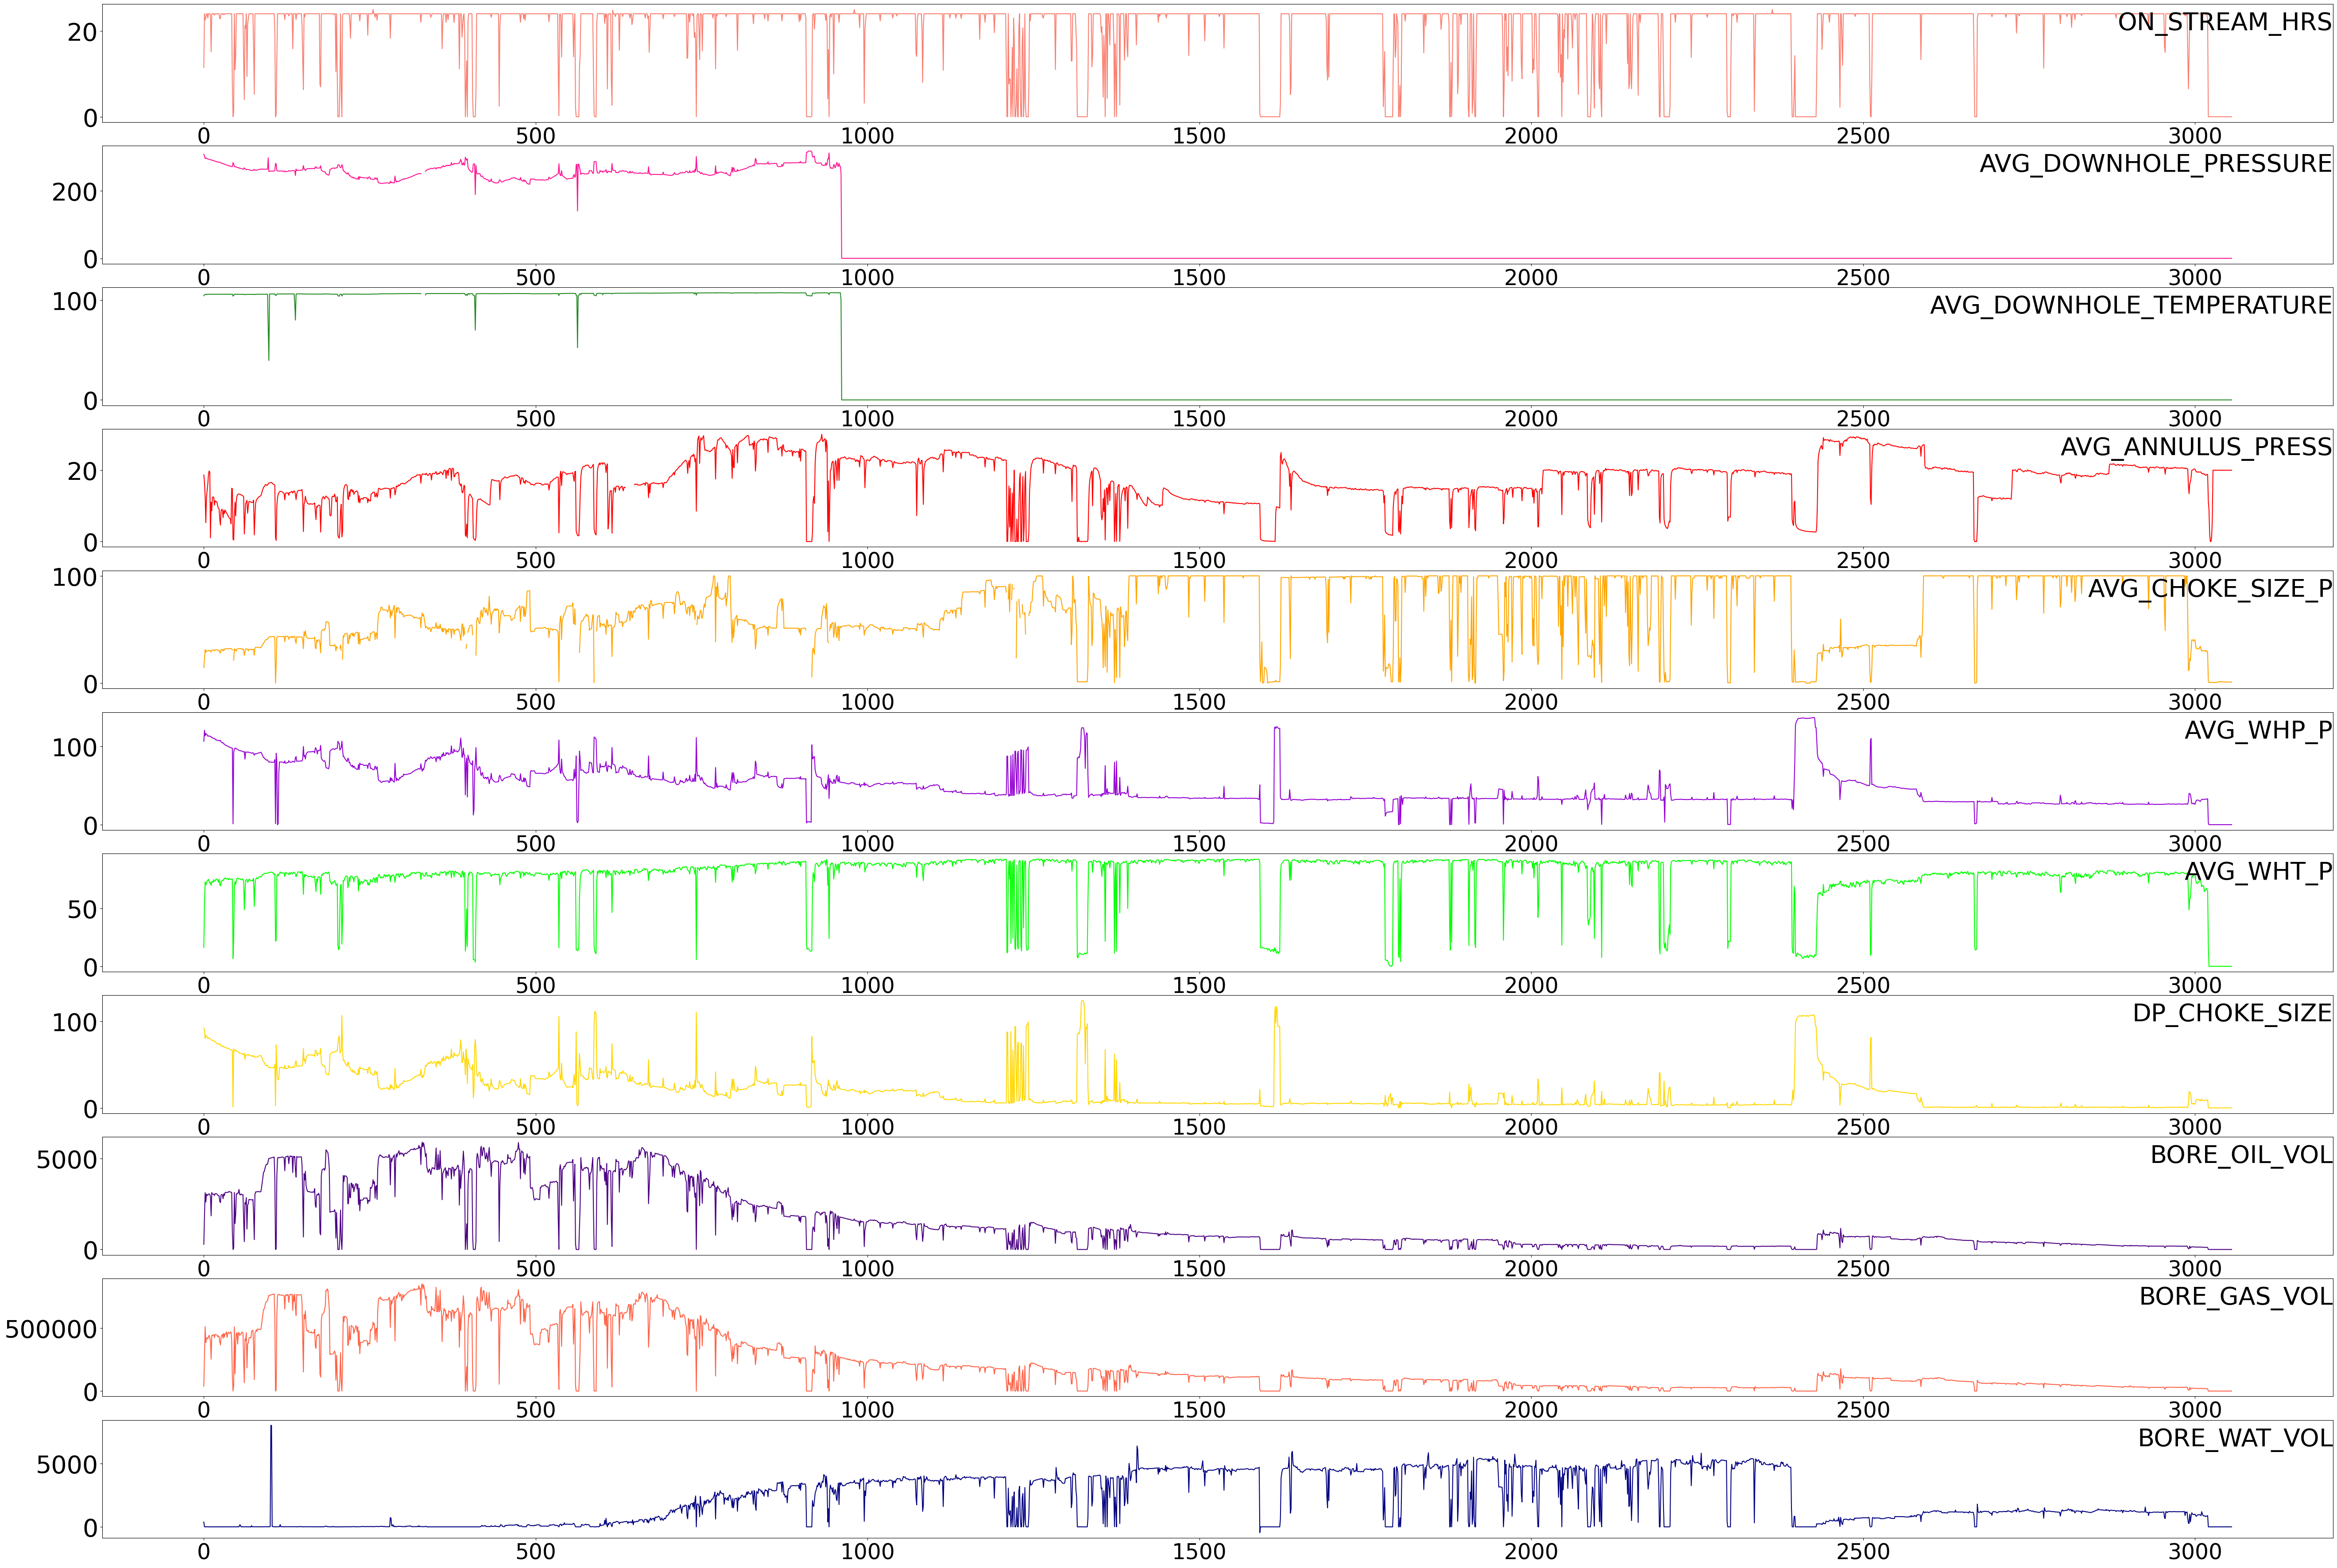
\includegraphics[width=1.0\textwidth]{images/Features3.png}
    \caption{Time series available to be used in the forecasting process.}
    \label{fig:all_features}
\end{figure}


Table with all the variables used in the model.

\begin{center}
\begin{tabular}{ |c|c|c|c| } 
%##############################################
% INFORMACOES PARA PREENCHER A TABELA
% https://discovervolve.com/2020/04/02/__how_to_access_volve/#Production-data_content
%#############################################
\hline
Column name & Type & Definition \\
\hline
% \multirow{3}{4em}{Multiple row} & cell2 & cell3 \\ 
DATEPRD & Data time & Date of production \\ 
ON$\_$STREAM$\_$HRS & Float & Onstream hours  \\ 
AVG$\_$DP$\_$TUBING & Float & Average of pressure differential in tubing \\ 
AVG$\_$CHOKE$\_$SIZE$\_$P & Float & Average of choke size                \\ 
AVG$\_$WHP$\_$P & Float & Average of well head pressure                  \\ 
AVG$\_$WHT$\_$P & Float & Average of well head temperature               \\ 
D$\_$CHOKE$\_$SIZE & Float & Choke size \\ 
BORE$\_$OIL$\_$VOL & Float & Volumetric data for produced oil \\ 
BORE$\_$GAS$\_$VOL & Float & Volumetric data for produced gas \\ 
BORE$\_$WAT$\_$VOL & Float & Volumetric data for produced water \\
\hline
\end{tabular}
\label{tab:Features}
\end{center}

\begin{figure}[h!]
    \centering
    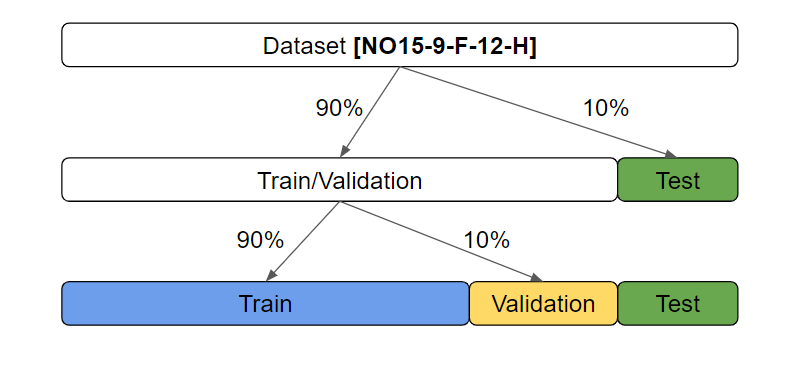
\includegraphics[width=0.6\textwidth]{images/dataset_split.png}
    \caption{Scheme of the split of the dataset in a train, validation, and test subsets.}
    \label{fig:data_split}
\end{figure}
\section{Extreme gradient boosting}
\label{sec:XGBoost}

According to Zhi-Hua Zhou\cite{zhou2012ensemble}, boosting algorithms are a group of algorithms that sequentially applies weak learners to achieve strong learning by the end. The extreme gradient boosting\cite{chen2016xgboost} is an optimized implementation of the gradient boosting framework proposed by Friedman et al.\cite{friedman2000additive},\cite{friedman2001greedy}. In this algorithm, each weak learn is made by a decision tree,
\section{Results}
\label{sec:Results}

\subsection{Dataset scaling type's effects}
Many machine learning algorithms perform better when numerical input variables are scaled to a standard range.

Fizemos três diferentes avaliações. Tendo como referência um lag de 5, avaliamos a influência causada pelos diferentes tipos de transformações utilizadas para escalar os dados.


\begin{center}
\begin{tabular}{ |c|c|c|c|c|c| } 
\hline
Type & Validation RMSE & Validation MAE & Test RMSE & Test MAE \\
\hline
% \multirow{3}{4em}{Multiple row} & cell2 & cell3 \\ 
MinMaxScaler & 0.03555 & 0.01364 & 0.0065 & 0.00459 \\ 
RobustScaler & 0.09398 & 0.03578 & 0.01789 & 0.01354 \\
StandardScaler & 0.13415 & 0.04909 & 0.03254 & 0.02179 \\
\hline
\end{tabular}
\label{tab:scaling_type}
\end{center}

Como podemos observar na tabela \ref{tab:scaling_type}, fazendo a transformação por meio da função de minmax, temos os melhores resultados nos dados de validação e também nos dados de teste.

\subsection{Impact of the quantity of data lags}

\begin{figure}[h!]
    \centering
    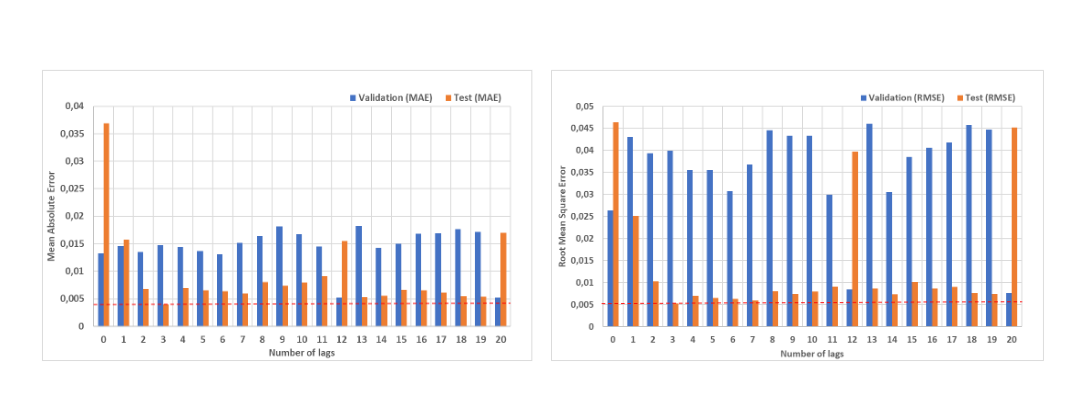
\includegraphics[width=1.0\textwidth]{images/Lag_metrics.png}
    \caption{Lag metrics}
    \label{fig:lag_metrics}
\end{figure}

\begin{figure}[h!]
    \centering
    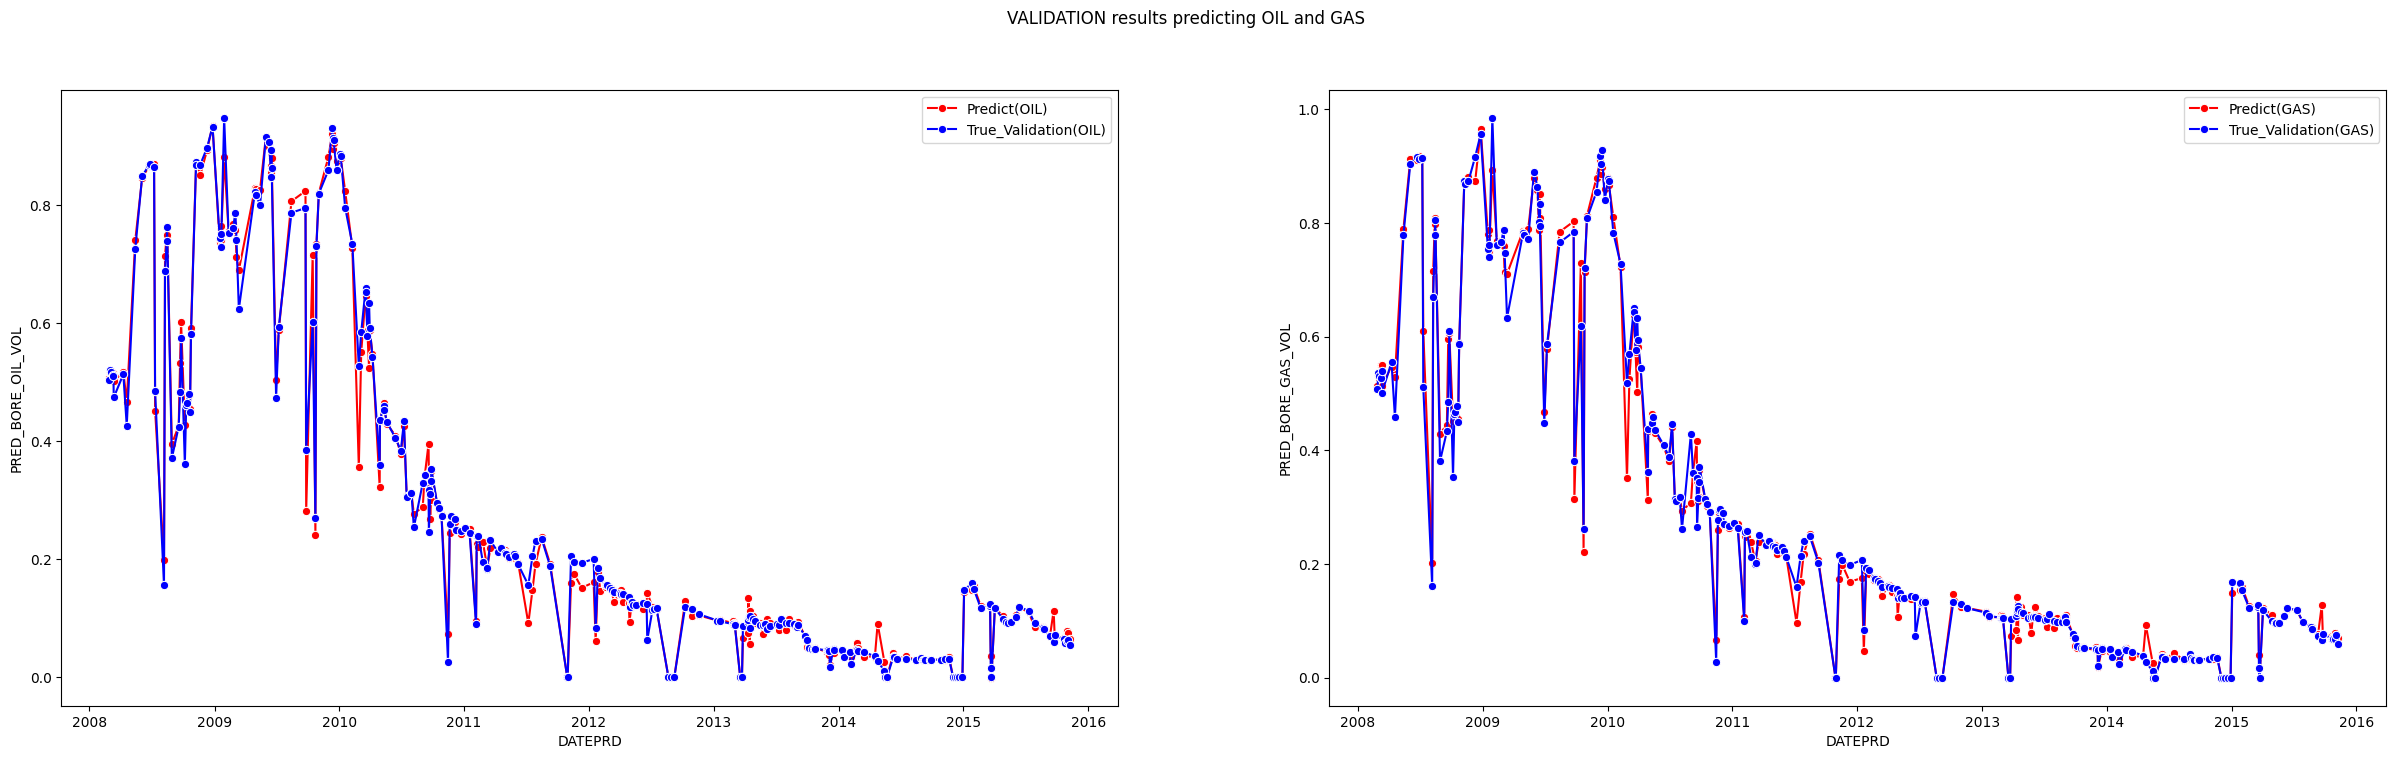
\includegraphics[width=1.0\textwidth]{images/Validation_lag_0.png}
    \caption{Validation 0}
    \label{fig:Val_0}
\end{figure}

\begin{figure}[h!]
    \centering
    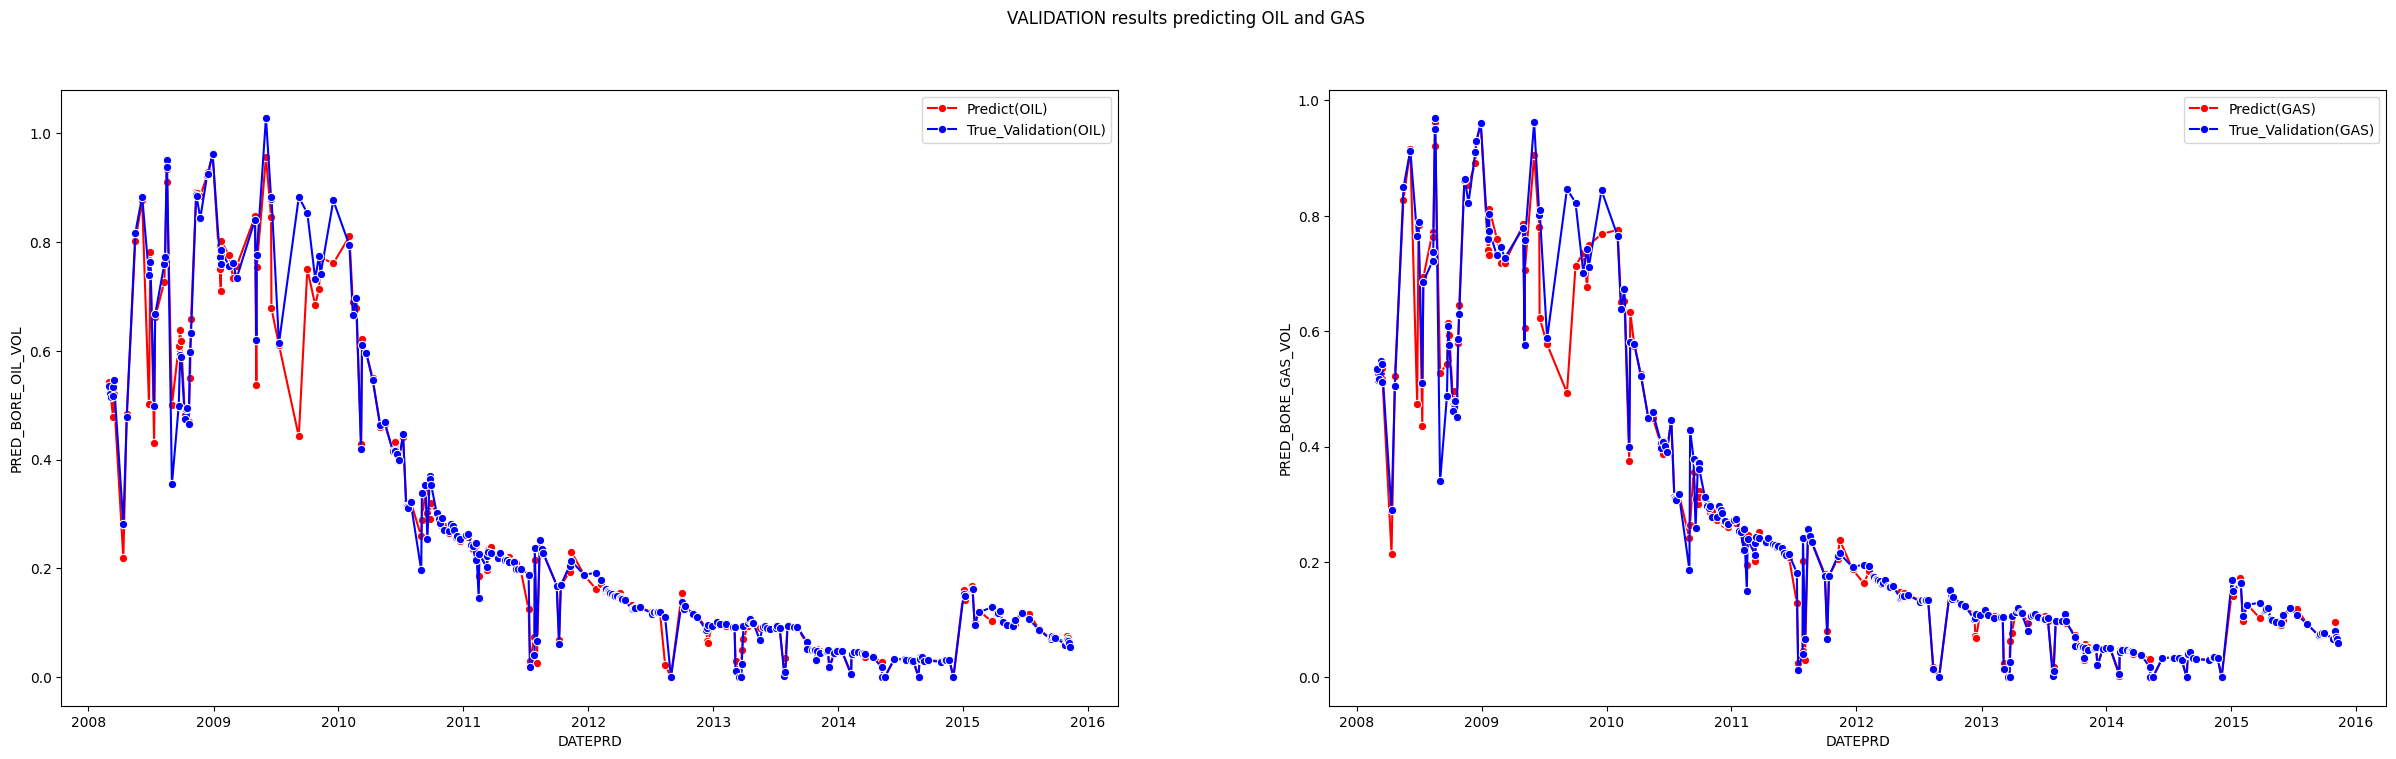
\includegraphics[width=1.0\textwidth]{images/Validation_lag_3.png}
    \caption{Validation 3}
    \label{fig:Val_3}
\end{figure}

\begin{figure}[h!]
    \centering
    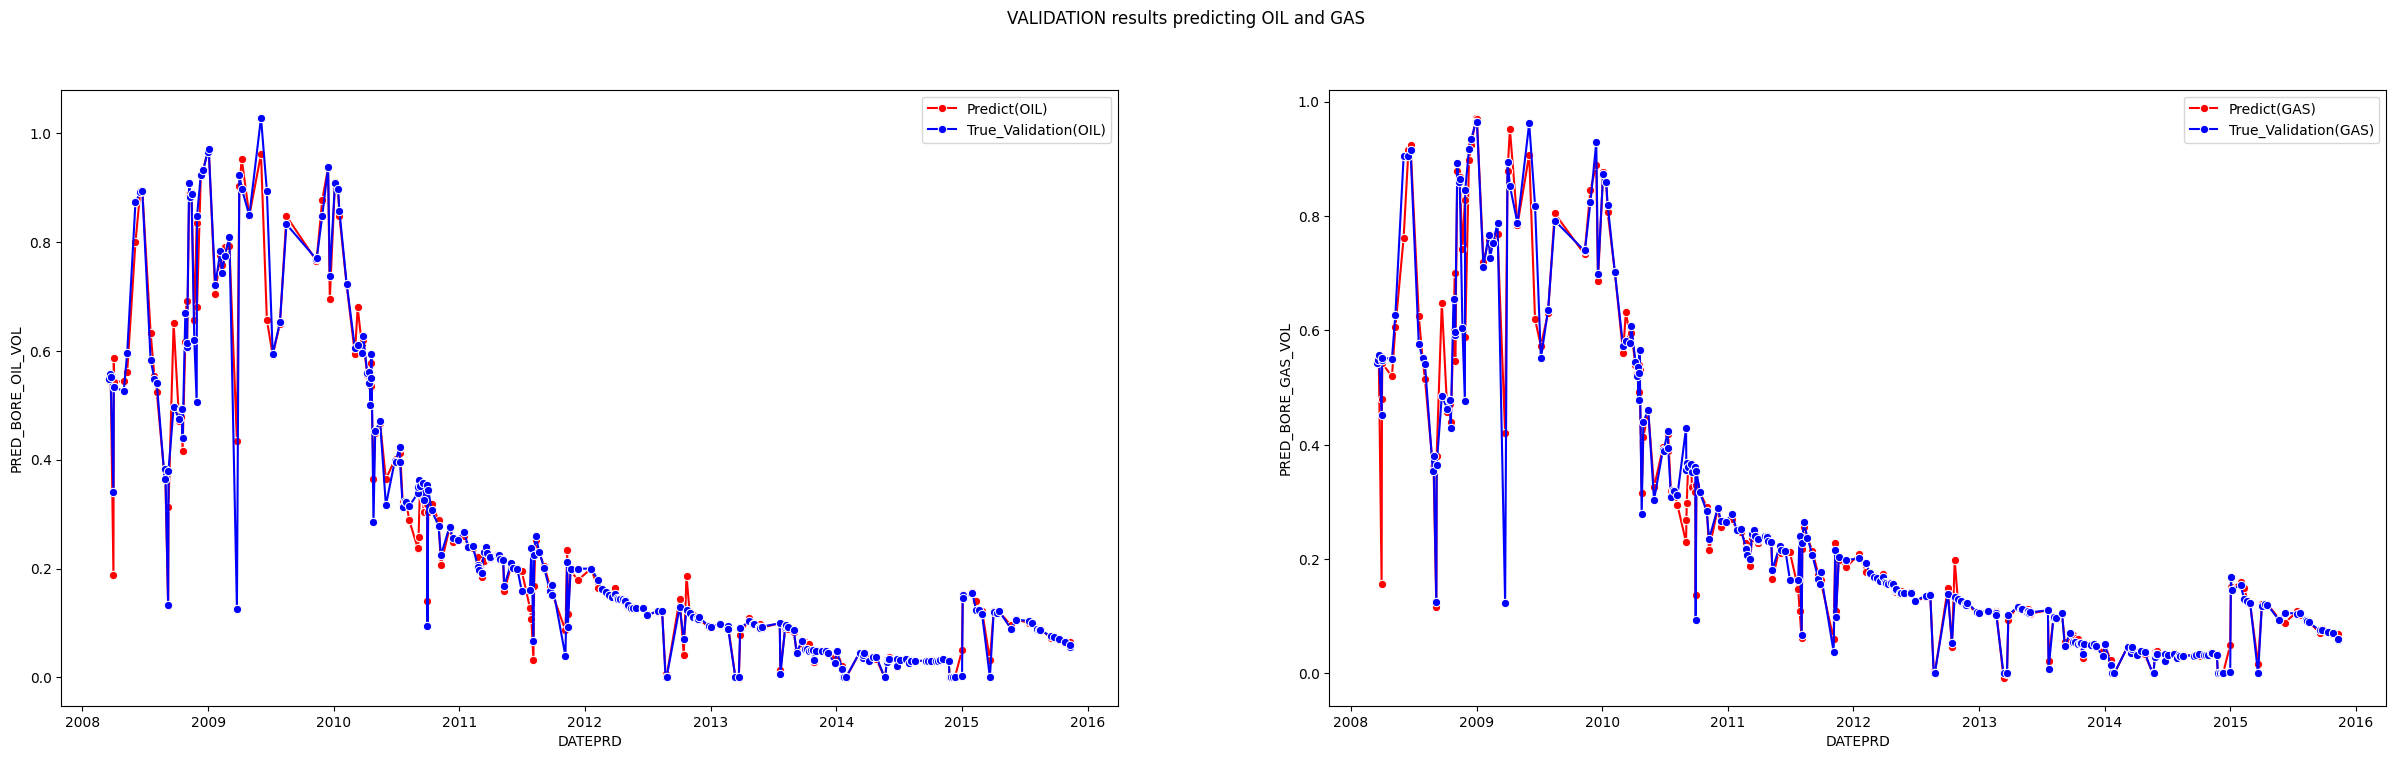
\includegraphics[width=1.0\textwidth]{images/Validation_lag_20.png}
    \caption{Validation 20}
    \label{fig:Val_20}
\end{figure}


\begin{figure}[h!]
    \centering
    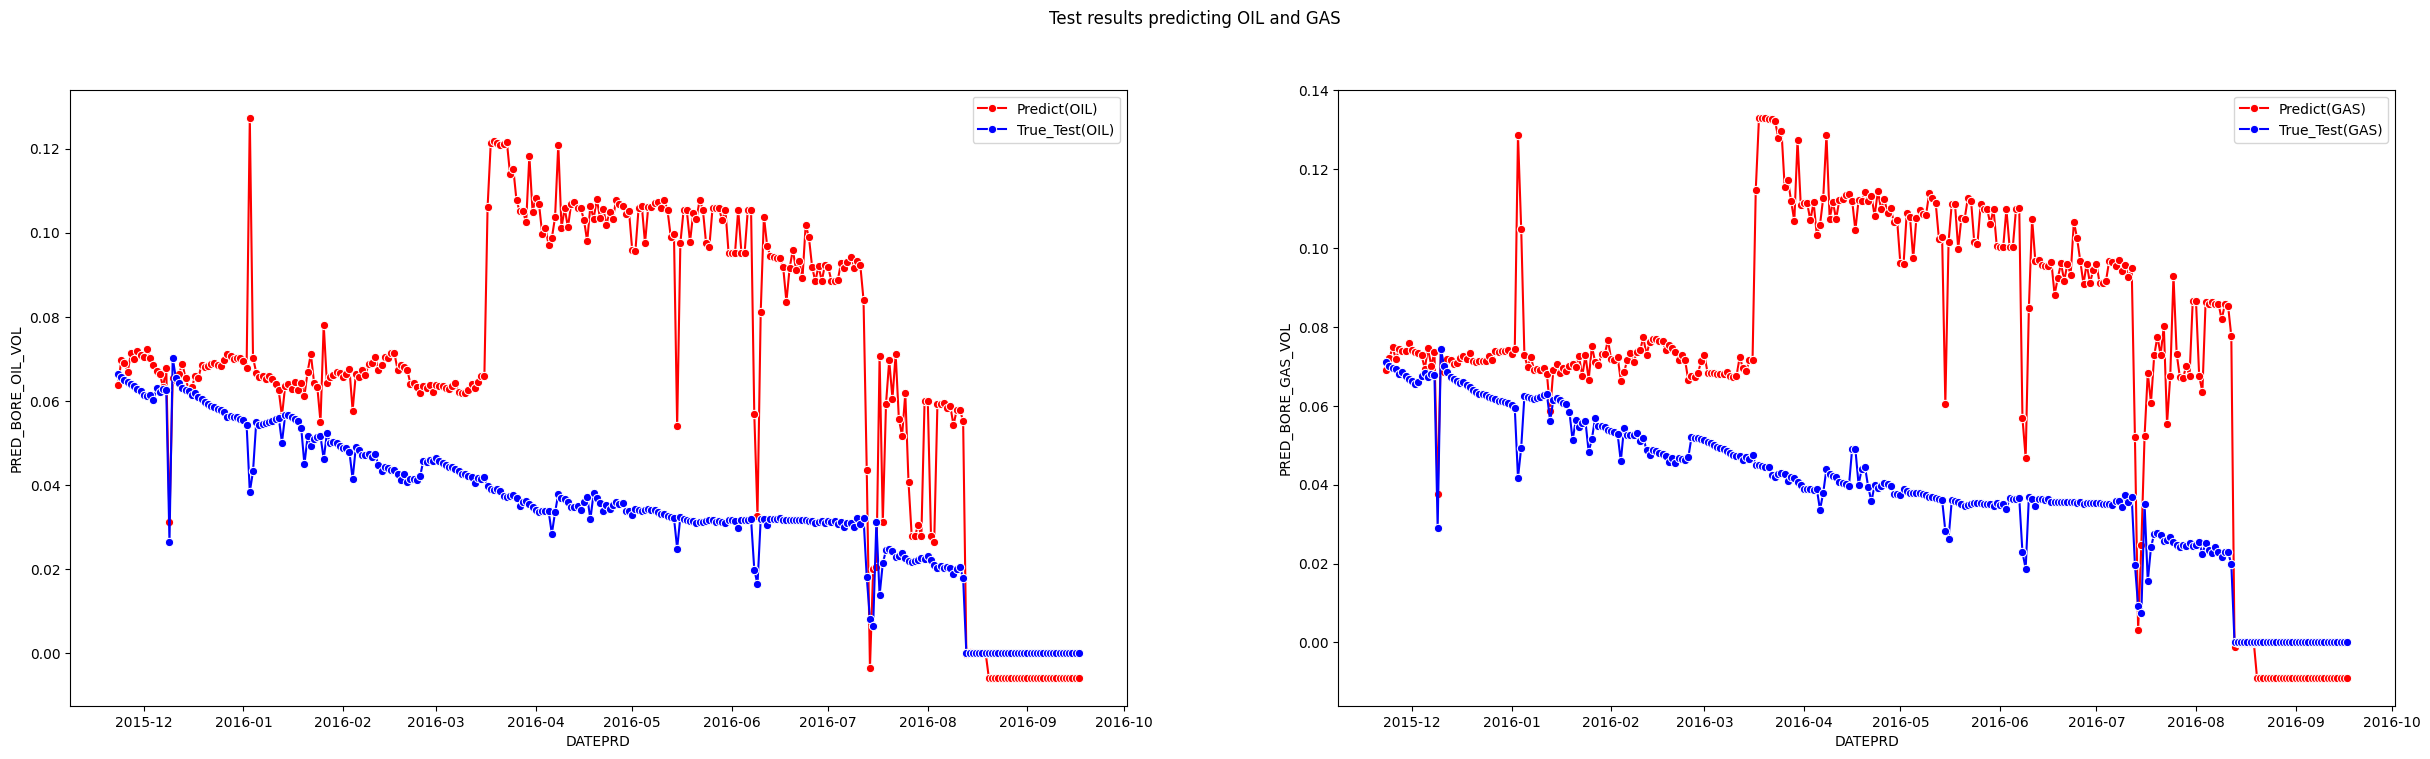
\includegraphics[width=1.0\textwidth]{images/Teste_lag_0.png}
    \caption{Test 0}
    \label{fig:Test_0}
\end{figure}

\begin{figure}[h!]
    \centering
    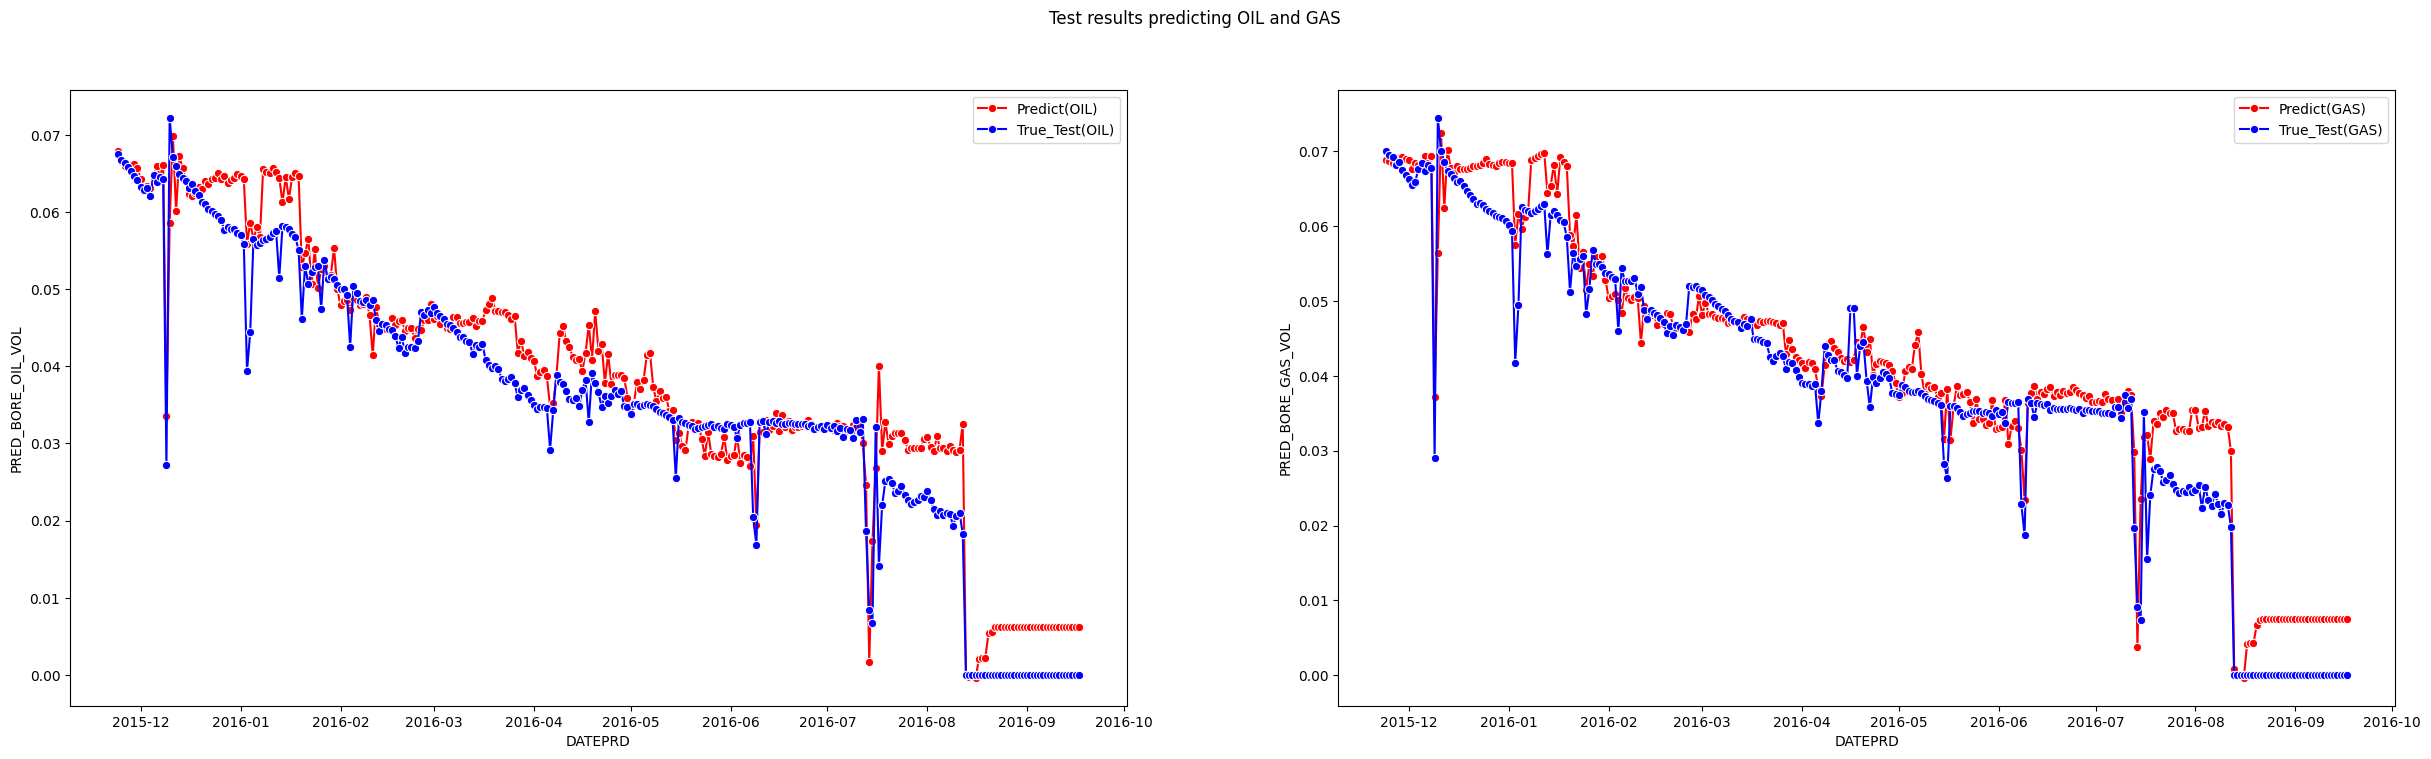
\includegraphics[width=1.0\textwidth]{images/Teste_lag_3.png}
    \caption{Test 3}
    \label{fig:Test_3}
\end{figure}

\begin{figure}[h!]
    \centering
    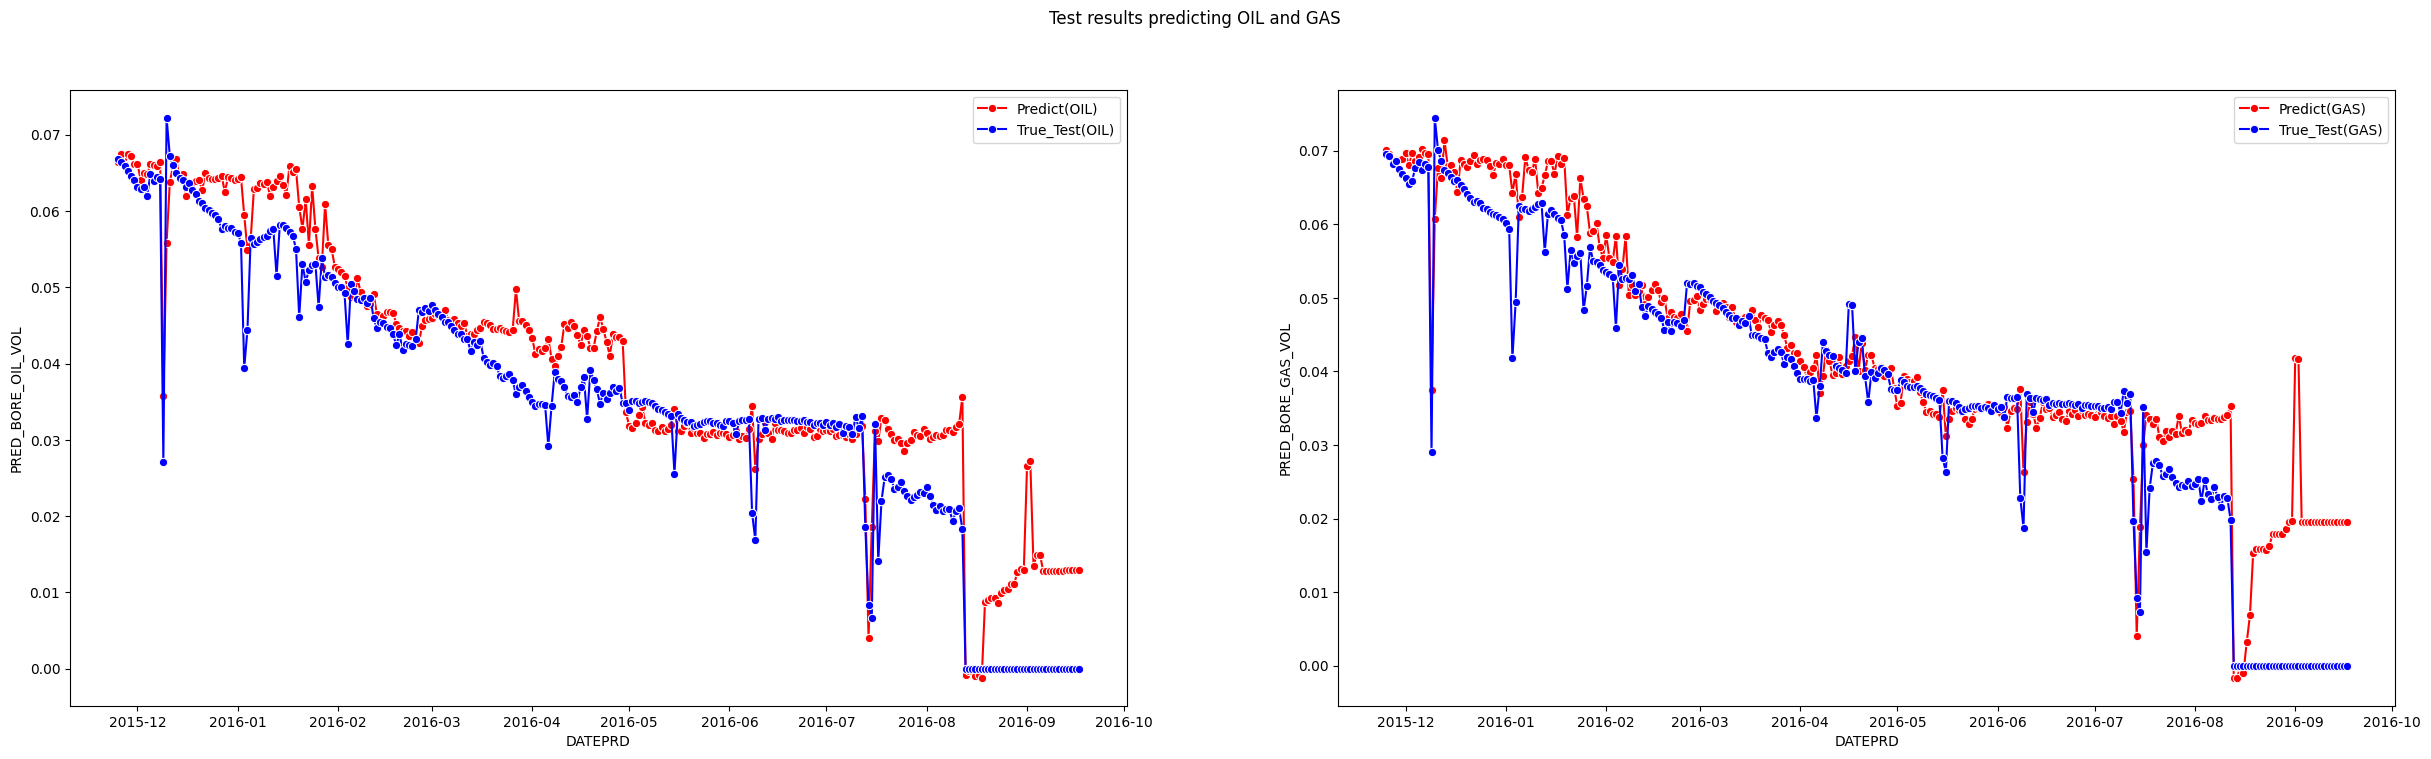
\includegraphics[width=1.0\textwidth]{images/Teste_lag_20.png}
    \caption{Test 20}
    \label{fig:Test_20}
\end{figure}
\section{Conclusions and discussions}
\label{sec:Conclusions}


Colocar aqui que o método foi capaz de fazer boas estimativas. 

Para melhores modelos seria necessário avaliar modelos de deep learning.
Fazer um melhor processamento de dados e não apenas fazer o drop dos dados de entrada.
% \section{Labels}
\label{sec:Labels}


I. Introduction 
\\
A. Background information about oil and gas production
\\
B. Explanation of Xgboost 
\\
C. Purpose of the essay

II. Xgboost in Oil and Gas Production Forecasting 
\\
A. Explanation of how Xgboost is used to forecast oil and gas production 
\\
B. Advantages of using Xgboost for forecasting 
\\
C. Challenges to using Xgboost for forecasting


III. Case Study: Application of Xgboost in Oil and Gas Production Forecasting
\\
A. Overview of the case study 
\\
B. Data collection methods 
\\
C. Results from the application of Xgboost in forecasting

IV. Comparison with Other Methods Used in Oil and Gas Production Forecasting
\\
A. Explanation of other methods used in forecasting oil and gas production 
\\
B. Comparison between Xgboost and other methods used in forecasting 
\\
C. Advantages and disadvantages of each method

V. Conclusion 
\\
A.Summary of key points discussed in the essay 
\\
B.Implication for future research on oil and gas production forecasting using machine learning models such as xGBoost.
\\
C.Concluding remarks on the importance of xGBoost in improving accuracy, speed, efficiency, reliability, cost-effectiveness, etc.,in oil and gas production forecasts

% \section{TASK_AI}
\label{sec:TASK_AI}

The oil and gas industry has been around for centuries and is crucial to the world's economy. Prediction in this industry can help optimize production and reduce costs. Machine learning models such as XGBoost have proven to be powerful tools for predicting oil and gas production. XGBoost is a tree-based ensemble model that excels at predicting values and is commonly used in industry.


Oil and gas production is one of the essential industries that drives the global economy.
The process of forecasting oil and gas production plays a vital role in the industry's success, as it
enables companies to plan for future operations, optimize resources, and enhance efficiency
while reducing costs. In this essay, we will discuss how XGBoost algorithm can be utilized in oil
and gas production forecast.

Machine learning techniques have gained significant attention in various industries due to
their ability to learn from data patterns without being explicitly programmed. In the oil and gas
industry, machine learning algorithms aid in decision-making processes by analyzing complex
datasets collected during drilling operations. XGBoost is one such algorithm that has been
widely used for its accuracy and speed.

Previous studies have shown promising results using XGBoost for oil and gas production
forecasting. For instance, Zhang et al.(2019) applied XGBoost on field data obtained from a
shale reservoir to estimate cumulative oil production with high accuracy levels. Similarly, Gao et
al.(2020) utilized an improved version of XGBoost called LightGBM on historical data from
several wells to predict daily oil output with satisfactory outcomes.


To implement XGBoost algorithm for forecasting purposes, relevant data must first be
collected from different sources such as drilling logs or geological surveys. This information is
then processed through specific techniques like normalization or imputation to ensure accuracy
before being fed into the model.

The results obtained from implementing the XGBoost algorithm are interpreted based on
factors such as Mean Absolute Error (MAE), Root Mean Squared Error (RMSE), or R-Squared
(R2) values. Comparing these outputs with previous studies' findings helps determine whether
our implementation was successful or not.

In conclusion, utilizing machine learning techniques like XGBoost for forecasting oil and
gas production is an efficient method that can significantly impact the industry's success rate
positively. Future work should focus on more extensive data collection processes coupled with
enhanced preprocessing techniques to improve model accuracy levels. Ultimately, optimizing the
industry's production processes will lead to cost reduction, improved efficiency, and increased
profitability
% \section{Informations}
\label{sec:Informations}

\textbf{XGBoost: A Scalable Tree Boosting System}

Tree boosting is a highly effective and widely used machine learning method. In this paper, we describe a scalable end-to-end tree boosting system called XGBoost, which is used widely by data scientists to achieve state-of-the-art results on many machine learning challenges. We propose a novel sparsity-aware algorithm for sparse data and weighted quantile sketch for approximate tree learning. More importantly, we provide insights on cache access patterns, data compression and sharding to build a scalable tree boosting system. By combining these insights, XGBoost scales beyond billions of examples using far fewer resources than existing system


\\

\textbf{A Simple and Fast Baseline for Tuning Large XGBoost Models}


XGBoost, a scalable tree-boosting algorithm, has proven effective for many prediction tasks of practical interest, especially using tabular datasets. Hyperparameter tuning can further improve the predictive performance, but unlike neural networks, full-batch training of many models on large datasets can be time consuming. Owing to the discovery that (i) there is a strong linear relation between dataset
size & training time, (ii) XGBoost models satisfy the ranking hypothesis, and (iii) lower-fidelity models can discover promising hyperparameter configurations, we show that uniform subsampling makes for a simple yet fast baseline to speed up the tuning of large XGBoost models using multi-fidelity hyperparameter optimization with data subsets as the fidelity dimension. We demonstrate the effectiveness
of this baseline on large-scale tabular datasets ranging from 15 − 70GB in size.

\\

\textbf{Solving problems of the oil and gas sector using machine learning algorithms}

The article describes the tasks of the oil and gas sector that can be
solved by machine learning algorithms. These tasks include the
study of the interference of wells, the classification of wells
according to their technological and geophysical characteristics, the
assessment of the effectiveness of ongoing and planned geological
and technical measures, the forecast of oil production for individual
wells and the total oil production for a group of wells, the forecast
of the base level of oil production, the forecast of reservoir
pressures and mapping. For each task, the features of building
machine learning models and examples of input data are described.
All of the above tasks are related to regression or classification
problems. Of particular interest is the issue of well placement
optimisation. Such a task cannot be directly solved using a single
neural network. It can be attributed to the problems of optimal
control theory, which are usually solved using dynamic
programming methods. A paper is considered where field
management and well placement are based on a reinforcement
learning algorithm with Markov chains and Bellman's optimality
equation. The disadvantages of the proposed approach are revealed.
To eliminate them, a new approach of reinforcement learning based
on the Alpha Zero algorithm is proposed. This algorithm is best
known in the field of gaming artificial intelligence, beating the
world champions in chess and Go. It combines the properties of
dynamic and stochastic programming. The article discusses in detail
the principle of operation of the algorithm and identifies common
features that make it possible to consider this algorithm as a
possible promising solution for the problem of optimising the
placement of a grid of wells. 

\\

\textbf{Performing Predictive Analysis using Machine Learning on the Information Retrieved from Production Data of Oil & Gas Upstream Segment}

Abstract—Machine learning is an area of knowledge, which
supports many of the established and reliable techniques in
Artificial intelligence. Oil and gas industry involve many sensors
to collect data continuously. Especially the main focus, is on the
Production data which will help the industry to perform
Predictive analysis that will forecast what outputs we may get in
future. The current research work focuses on the data produced
from an oil well, over a month and then tries to predict the
average oil rate, based on certain elements. In order to perform
this, a predictive tool RapidMiner is used, and Regression model
is applied. This research work helps in predicting the most
dependent factor on the predictive variable, which is Average Oil
Rate. 

\\
\textbf{Crude oil price forecasting using XGBoost}

Abstract—One of the most important role of economic
variables in today's world countries are the price and the change
of the price of crude oil. Changes in the price of crude oil have a
very critical role in terms of treasury and budget, both in
company and state planning. For example, one may choose one of
the energy or natural gas indexed energy production plans based
on the trend of the crude oil price, for planning to meet the need
for electricity next year. Accurate forecasting of the crude oil
price and realization of the forecasts based on this forecast will
provide savings or gains in government and corporate economies,
which can reach billions of dollars. There is a great need for this
estimation in countries where crude oil production is low and
heavily dependent on crude oil import. In this paper, the
parameters which are the factors affecting the crude oil prices
will be interpreted using XGBoost, a gradient boosting model,
from machine learning libraries and estimation will be made.

\\
\textbf{Well Performance Classification and Prediction: Deep Learning and Machine Learning Long Term Regression Experiments on Oil, Gas, and Water Production}

In the oil and gas industries, predicting and classifying oil and gas production for hydrocarbon wells is difficult. Most oil and gas companies use reservoir simulation software to predict future
oil and gas production and devise optimum field development plans. However, this process costs an
immense number of resources and is time consuming. Each reservoir prediction experiment needs
tens or hundreds of simulation runs, taking several hours or days to finish. In this paper, we attempt
to overcome these issues by creating machine learning and deep learning models to expedite the
process of forecasting oil and gas production. The dataset was provided by the leading oil producer,
Saudi Aramco. Our approach reduced the time costs to a worst-case of a few minutes. Our study
covered eight different ML and DL experiments and achieved its most outstanding R2 scores of 0.96
for XGBoost, 0.97 for ANN, and 0.98 for RNN over the other experiments.

\\

\textbf{Application of Machine Learning Method of Data-Driven Deep Learning Model to Predict Well Production Rate in the Shale Gas Reservoirs}

Reservoir modeling to predict shale reservoir productivity is considerably uncertain and
time consuming. Since we need to simulate the physical phenomenon of multi-stage hydraulic
fracturing. To overcome these limitations, this paper presents an alternative proxy model based
on data-driven deep learning model. Furthermore, this study not only proposes the development
process of a proxy model, but also verifies using field data for 1239 horizontal wells from the Montney
shale formation in Alberta, Canada. A deep neural network (DNN) based on multi-layer perceptron
was applied to predict the cumulative gas production as the dependent variable. The independent
variable is largely divided into four types: well information, completion and hydraulic fracturing
and production data. It was found that the prediction performance was better when using a principal
component with a cumulative contribution of 85% using principal component analysis that extracts
important information from multivariate data, and when predicting with a DNN model using 6
variables calculated through variable importance analysis. Hence, to develop a reliable deep learning
model, sensitivity analysis of hyperparameters was performed to determine one-hot encoding,
dropout, activation function, learning rate, hidden layer number and neuron number. As a result, the
best prediction of the mean absolute percentage error of the cumulative gas production improved
to at least 0.2% and up to 9.1%. The novel approach of this study can also be applied to other shale
formations. Furthermore, a useful guide for economic analysis and future development plans of
nearby reservoirs

\\

\textbf{Modified aquila optimizer for forecasting oil production}


Oil production estimation plays a critical role in economic plans for local governments and organizations. Therefore, many studies applied different Artificial Intelligence (AI) based methods to estimate oil production in different countries. The Adaptive Neuro-Fuzzy Inference System (ANFIS) is a well-known model that has been successfully employed in various applications, including time-series forecasting. However, the ANFIS model faces critical shortcomings in its parameters during the configuration process. From this point, this paper works to solve the drawbacks of the ANFIS by optimizing ANFIS parameters using a modified Aquila Optimizer (AO) with the Opposition-Based Learning (OBL) technique. The main idea of the developed model, AOOBL-ANFIS, is to enhance the search process of the AO and use the AOOBL to boost the performance of the ANFIS. The proposed model is evaluated using real-world oil production datasets collected from different oilfields using several performance metrics, including Root Mean Square Error (RMSE), Mean Absolute Error (MAE), coefficient of determination (R2), Standard Deviation (Std), and computational time. Moreover, the AOOBL-ANFIS model is compared to several modified ANFIS models include Particle Swarm Optimization (PSO)-ANFIS, Grey Wolf Optimizer (GWO)-ANFIS, Sine Cosine Algorithm (SCA)-ANFIS, Slime Mold Algorithm (SMA)-ANFIS, and Genetic Algorithm (GA)-ANFIS, respectively. Additionally, it is compared to well-known time series forecasting methods, namely, Autoregressive Integrated Moving Average (ARIMA), Long Short-Term Memory (LSTM), Seasonal Autoregressive Integrated Moving Average (SARIMA), and Neural Network (NN). The outcomes verified the high performance of the AOOBL-ANFIS, which outperformed the classic ANFIS model and the compared models.

\\

\textbf{Forecasting oil production using ensemble empirical model decomposition based Long Short-Term Memory neural network}

Oil production forecasting is an important means of understanding and effectively developing reservoirs. Reservoir numerical simulation is the most mature and effective method for production forecasting, but its accuracy mostly depends on high-quality history matching and accurate geological models. In order to achieve fast and accurate production predicting, an ensemble empirical mode decomposition (EEMD) based Long Short-Term Memory (LSTM) learning paradigm is proposed for oil production forecasting. In this paper, the original oil production series are first split into training set and test set. The data of test set is gradually added to the training set and decomposed by EEMD to obtain multiple intrinsic mode functions (IMFs). The stability of IMFs is analyzed by its Means and curve similarity computed by Dynamic time warping (DTW). Then proper number of stable IMFs are selected as predictor variables for machine learning. Considering the variation trend and context information of production series, LSTM is utilized to establish predictive model for production forecasting. The optimal hyper-parameters of LSTM are determined by Genetic algorithm (GA). For evaluation and verification purpose, the proposed model is applied to two actual oilfields from China. Empirical results demonstrated that the proposed approach is capable of giving almost perfect production forecasting.



\\

\textbf{A comparative machine learning study for time series oil production forecasting: ARIMA, LSTM, and Prophet}

It is challenging to predict the production performance of unconventional reservoirs because of the sediment heterogeneity, intricate flow channels, and complex fluid phase behavior. The traditional oil production prediction methods (e.g., decline curve analysis and reservoir simulation modeling forecasting) are subjective. This paper presents a machine learning-based time series forecasting method, which considers the existing data as time series and extracts the salient characteristics of historical data to predict values of a future time sequence. We used time series forecasting because of the historical fluctuations in production well and reservoir operations. Three algorithms were studied and compared to address the limitations of traditional production forecasting: Auto-Regressive Integrated Moving Averages (ARIMA), Long-Short-Term Memory (LSTM) network, and Prophet. This study starts with the representative oil production data from a well located in an unconventional reservoir in the Denver-Julesburg (DJ) Basin. 70% of the data was used for model training, whereas the remaining 30% of data was used to evaluate the performance of the above-mentioned methods. Then, the decline curve analysis and reservoir simulation modeling forecasting were applied for comparison. The advantages of the machine-learning models include a simple workflow, no prior assumption about the reservoir type, fast prediction, and reliable performance prediction for a typical fluctuating declining curve. More importantly, the ‘Prophet’ model captures production fluctuation caused by winter impact, which can attract the operator's attention and prevent potential failures. This has rarely been explored and discussed by previous studies. The application of ARIMA, LSTM, and Prophet methods to 65 wells in the DJ Basin show that ARIMA and LSTM perform better than Prophet—probably because not all oil production data include seasonal influences. Furthermore, the wells in the nearby pads can be studied using the same parameter values in ARIMA and LSTM for predicting oil prediction in a transferred learning framework. Specifically, we observed that ARIMA is robust in predicting the oil production rate of wells across the DJ Basin.
%% The Appendices part is started with the command \appendix;
%% appendix sections are then done as normal sections
%% \appendix

%% \section{}
%% \label{}

%% If you have bibdatabase file and want bibtex to generate the
%% bibitems, please use
%%
%%  \bibliographystyle{elsarticle-harv} 
%%  \bibliography{<your bibdatabase>}

%% else use the following coding to input the bibitems directly in the
%% TeX file.

% \begin{thebibliography}{00}

% %% \bibitem[Author(year)]{label}
% %% Text of bibliographic item

% \bibitem[ ()]{}

% \end{thebibliography}

\bibliographystyle{elsarticle-harv} 
\bibliography{bibfile}
\end{document}

\endinput
%%
%% End of file `elsarticle-template-harv.tex'.
